\documentclass[ignorenonframetext,]{beamer}
\setbeamertemplate{caption}[numbered]
\setbeamertemplate{caption label separator}{:}
\setbeamercolor{caption name}{fg=normal text.fg}
\usepackage{amssymb,amsmath}
\usepackage{ifxetex,ifluatex}
\usepackage{fixltx2e} % provides \textsubscript
\usepackage{lmodern}
\ifxetex
  \usepackage{fontspec,xltxtra,xunicode}
  \defaultfontfeatures{Mapping=tex-text,Scale=MatchLowercase}
  \newcommand{\euro}{€}
\else
  \ifluatex
    \usepackage{fontspec}
    \defaultfontfeatures{Mapping=tex-text,Scale=MatchLowercase}
    \newcommand{\euro}{€}
  \else
    \usepackage[T1]{fontenc}
    \usepackage[utf8]{inputenc}
      \fi
\fi
% use upquote if available, for straight quotes in verbatim environments
\IfFileExists{upquote.sty}{\usepackage{upquote}}{}
% use microtype if available
\IfFileExists{microtype.sty}{\usepackage{microtype}}{}
\usepackage{longtable,booktabs}
\usepackage{caption}
% These lines are needed to make table captions work with longtable:
\makeatletter
\def\fnum@table{\tablename~\thetable}
\makeatother
\usepackage{graphicx}
\makeatletter
\def\maxwidth{\ifdim\Gin@nat@width>\linewidth\linewidth\else\Gin@nat@width\fi}
\def\maxheight{\ifdim\Gin@nat@height>\textheight0.8\textheight\else\Gin@nat@height\fi}
\makeatother
% Scale images if necessary, so that they will not overflow the page
% margins by default, and it is still possible to overwrite the defaults
% using explicit options in \includegraphics[width, height, ...]{}
\setkeys{Gin}{width=\maxwidth,height=\maxheight,keepaspectratio}

% Comment these out if you don't want a slide with just the
% part/section/subsection/subsubsection title:
\AtBeginPart{
  \let\insertpartnumber\relax
  \let\partname\relax
  \frame{\partpage}
}
\AtBeginSection{
  \let\insertsectionnumber\relax
  \let\sectionname\relax
  \frame{\sectionpage}
}
\AtBeginSubsection{
  \let\insertsubsectionnumber\relax
  \let\subsectionname\relax
  \frame{\subsectionpage}
}

\setlength{\parindent}{0pt}
\setlength{\parskip}{6pt plus 2pt minus 1pt}
\setlength{\emergencystretch}{3em}  % prevent overfull lines
\setcounter{secnumdepth}{0}
\usepackage{minted}
\usemintedstyle{tango}
\newminted{haskell}{mathescape}
\newmintinline{haskell}{}
\setmonofont[Mapping=tex-text,Ligatures={TeX,Common,Contextual},Scale=MatchUppercase]{PragmataPro}
\setsansfont[Mapping=tex-text,Ligatures={TeX,Common,Contextual},Scale=MatchUppercase]{FreightSans Pro}

\title{The Math of Types}
\author{Ryan Orendorff}
\date{June 13th, 2015}

\begin{document}
\frame{\titlepage}

\begin{frame}[fragile]{What we will talk about today}

Time permitting, I would like to cover the following topics.

\begin{itemize}
\itemsep1pt\parskip0pt\parsep0pt
\item
  The math of regular data types.
\item
  What a zipper is, and why you might want one.
\item
  Dissection and delimited continuations (as time permits).
\end{itemize}

\long\def\ignore\#1\{\}

\ignore{

> module DiffBayhac where
>

}

\end{frame}

\section{The Math of Regular Data
Types}\label{the-math-of-regular-data-types}

\begin{frame}[fragile]{What is an Algebra?}

In the most general sense, ``algebra is the study of mathematical
symbols and the rules for manipulating these symbols''.\footnote<.->{https://en.wikipedia.org/wiki/Algebra}

Algebraic structures provide a way for us to ``bolt on'' manipulation
powers onto a set of symbols.

In this talk, we will consider symbols that are both numbers and types.

\end{frame}

\begin{frame}[fragile]{Magmas}

A magma is a binary function \(\otimes\) that takes two symbols and
produces a third from the same set of symbols.\footnote<.->{the fact it
  returns something from the same set makes the operation \emph{closed}}

\pause

For example, if the symbols we are dealing with are numbers, then we can
consider \(\cdot\) to be a binary operator that performs this property.

\pause

On types, one operation we can do to combine two types is to create a
pair, which is itself a type.

\begin{haskellcode}
data (,) a b = (a, b)
\end{haskellcode}

\end{frame}

\begin{frame}[fragile]{Monoids}

Monoids are similar to magmas. They need a binary operator, but it has
to have an identity element such that

\[
a \otimes 0 = 0 \otimes a = a
\]

\pause

Our multiplication on numbers still follows this rule if we choose 1 as
the identity element.

\[
a \cdot 1 = a
\]

\pause

On types, do we have the same property? Is there a \texttt{One}?

\[
(a, One) \simeq a
\]

\end{frame}

\begin{frame}[fragile]{Sidenote: This \emph{up to isomorphism} thing}

When we talk about something ``up to isomorphism'' for the types, we
mean that there is a way to convert between the types. Specifically, if

\begin{haskellcode}
f :: A -> B ; g :: B -> A
\end{haskellcode}

then

\begin{haskellcode}
f . g = id; g . f = id
\end{haskellcode}

\pause

For example, we define

\begin{haskellcode}
type A = (Int, (String, Int))
type B = ((Int, String), Int)

f (a, (b, c)) = ((a, b), c)
g ((a, b), c) = (a, (b, c))
\end{haskellcode}

We will use \(\simeq\) to mean ``equal by isomorphism''.

\end{frame}

\begin{frame}[fragile]{So what is \texttt{OneType}?}

We need a value that we can always pair with some \texttt{a} that does
not carry any information. What does this mean? I should be able to
write these functions.

\begin{haskellcode}
f :: (a, One) -> a
g :: a -> (a, One)
\end{haskellcode}

We need a type where there is only one way to make a value of it.

\pause

How about

\begin{haskellcode}
data One = One -- Also written as data () = ()
               --              or data Unit = Unit
\end{haskellcode}

\pause

\begin{haskellcode}
f (a, _) = a
g a = (a, One)
\end{haskellcode}

\end{frame}

\begin{frame}[fragile]{What we have so far}

\begin{longtable}[c]{@{}lll@{}}
\toprule
Operations & Numbers & Types\tabularnewline
\midrule
\endhead
\(\otimes\) & \(\cdot\) & \texttt{(,)}\tabularnewline
\(\otimes\) associativity &
\(a \cdot (b \cdot c) = (a \cdot b) \cdot c\) & \texttt{(a,\ (b,\ c))}
\(\simeq\) \texttt{((a,\ b),\ c)}\tabularnewline
\(\otimes\) identity & 1 & \texttt{One} or \texttt{()}\tabularnewline
\(\otimes\) identity law & \(a \cdot 1 = a\) & \texttt{(a,\ One)}
\(\simeq\) \texttt{a}\tabularnewline
\bottomrule
\end{longtable}

We didn't talk about associativity, but monoids must have it as well.

\pause

But I think we forgot something

\end{frame}

\begin{frame}[fragile]{What about addition?}

We can certainly add numbers as well, with the following properties

\[
\begin{aligned}
a + 0 = a \\
a + (b + c) = (a + b) + c
\end{aligned}
\]

\pause

Numbers form a monoid using the \texttt{+} operator.

Can we do sums with types?

\pause

What about

\begin{haskellcode}
data Either a b = Left a | Right b
\end{haskellcode}

\end{frame}

\begin{frame}[fragile]{Addition on Types}

Let's see if \texttt{Either} makes sense over the associativity
property.

\begin{haskellcode}
Either A (Either B C) == Either (Either A B) C
\end{haskellcode}

\pause

\begin{haskellcode}
f (Left a) = Left (Left a)
f (Right (Left b)) = Left (Right b)
f (Right (Right c)) = Right c
\end{haskellcode}

and \texttt{g} is defined similarly.

\end{frame}

\begin{frame}[fragile]{What is the identity element for addition?}

For numbers, it is 0. For types, we need something that can never
happen.

\pause

\begin{haskellcode}
data Void -- no data constructors
\end{haskellcode}

\pause

This means, for \texttt{Either\ a\ Void}, it is impossible to call the
\texttt{Right} constructor.

\pause

From this we can easily show \texttt{Either\ a\ Void} \(\simeq\)
\texttt{a}

\end{frame}

\begin{frame}[fragile]{The combined total of our investigation}

\begin{longtable}[c]{@{}lll@{}}
\toprule
Operations & Numbers & Types\tabularnewline
\midrule
\endhead
\(\otimes\) & \(\cdot\) & \texttt{(,)}\tabularnewline
\(\otimes\) associativity &
\(a \cdot (b \cdot c) = (a \cdot b) \cdot c\) & \texttt{(a,\ (b,\ c))}
\(\simeq\) \texttt{((a,\ b),\ c)}\tabularnewline
\(\otimes\) identity & 1 & \texttt{One} or \texttt{()}\tabularnewline
\(\otimes\) identity law & \(a \cdot 1 = a\) & \texttt{(a,\ One)}
\(\simeq\) \texttt{a}\tabularnewline
\(\oplus\) & \(+\) & \texttt{Either}\tabularnewline
\(\oplus\) associativity & \(a + (b + c) = (a + b) + c\) &
\texttt{Either\ A\ (Either\ B\ C)} \(\simeq\)\tabularnewline
& & \texttt{Either\ (Either\ A\ B)\ C}\tabularnewline
\(\oplus\) identity & 0 & \texttt{Void}\tabularnewline
\(\oplus\) identity law & \(a \cdot 0 = a\) & \texttt{Either\ a\ Void}
\(\simeq\) \texttt{a}\tabularnewline
\bottomrule
\end{longtable}

\end{frame}

\begin{frame}[fragile]{And there are a few other laws}

All of these laws are followed by numbers and types. This makes both
numbers and types an algebraic structure called a semiring.

\begin{longtable}[c]{@{}lll@{}}
\toprule
Operations & Numbers & Types\tabularnewline
\midrule
\endhead
\(\otimes\) commute & \(a \cdot b = b \cdot a\) & \texttt{(a,\ b)}
\(\simeq\) \texttt{(b,\ a)}\tabularnewline
\(\oplus\) commute & \(a + b = b + a\) & \texttt{Either\ A\ B}
\(\simeq\)\tabularnewline
& & \texttt{Either\ B\ A}\tabularnewline
\(\oplus\) implied equality & \(a + b = a + c\) & \texttt{Either\ A\ B}
\(\simeq\) \texttt{Either\ A\ C}\tabularnewline
& \(\implies b = c\) & \(\implies\) \texttt{B} \(\simeq\)
\texttt{C}\tabularnewline
Left distributive & \((a + b) \cdot c =\) & \texttt{(Either\ A\ B,\ C)}
\(\simeq\)\tabularnewline
& \(a \cdot c + b \cdot c\) &
\texttt{Either\ (A,\ C)\ (B,\ C)}\tabularnewline
Zero is not One & \(0 \neq 1\) & \texttt{Void} \(\not\simeq\)
\texttt{One}\tabularnewline
\bottomrule
\end{longtable}

\end{frame}

\begin{frame}[fragile]{How can we use this?}

Using the semiring operations, we can start to build up terms
programmatically.

For example, take the \texttt{Maybe} type.

\begin{haskellcode}
data Maybe a = Nothing | Just a
\end{haskellcode}

\pause

\begin{haskellcode}
type Maybe a = Either One a
\end{haskellcode}

\pause

In number this is \(Maybe(x) = 1 + x\)

\end{frame}

\begin{frame}[fragile]{Making the algebra easier to see}

\begin{haskellcode}
{-# LANGUAGE TypeOperators #-}
{-# LANGUAGE DeriveFunctor #-}

newtype K a x = K a deriving (Show, Functor)
newtype Id x = Id x deriving (Show, Functor)
newtype (p :*: q) x = Prod (p x, q x) deriving (Show, Functor)
data (p :+: q) x = L (p x) | R (q x) deriving (Show, Functor)

type One = K ()

one = K ()
\end{haskellcode}

The paper ``Algebra of Programming'' (Bird, de Moor 1997) has a much
more in depth coverage.\footnote<.->{Copied directly from the Clowns and
  Jokers paper}

\end{frame}

\begin{frame}[fragile]{Recreating Maybe}

\begin{haskellcode}
type Maybe = One :+: Id

just :: x -> Maybe x
just x = R (Id x)

nothing :: Maybe x
nothing = L one
\end{haskellcode}

\pause

\begin{haskellcode}
fmap (+2) nothing == L one
\end{haskellcode}

\pause

\begin{haskellcode}
fmap (+2) (just 5) == R (Id 7)
\end{haskellcode}

Notice no functor instance was declared for \texttt{Maybe}.

\end{frame}

\section{Zippers}\label{zippers}

\begin{frame}[fragile]{Motivation: Updating lists has poor performance}

Say you want to update one element of a list. Here is one way to do
that.

\begin{haskellcode}
-- Insanely partial
update :: Int -> (a -> a) -> [a] -> [a]
update index _ [] = error "Hey, I need something to edit dummy!"
update index f (x:xs) = if index == 0
                        then f x : xs
                        else x : update (index - 1) f xs
\end{haskellcode}

\pause

As an example, lets update an element of a simple list.

\begin{haskellcode}
update 2 (10 `const`) list == [1, 2, 10, 4, 5]
\end{haskellcode}

\end{frame}

\begin{frame}[fragile]{Where is the poor performance?}

Say we start with some list \texttt{l} with six elements.

\begin{haskellcode}
    index
    0   1   2   3   4   5
l = a : b : c : d : e : f : []
\end{haskellcode}

Now let's update the third element using some update function
\texttt{f}.

\end{frame}

\begin{frame}[fragile]{Where is the poor performance?}

Say we start with some list \texttt{l} with six elements.

\begin{haskellcode}
    index
    0   1   2   3   4   5
l = a : b : c : d : e : f : []
--                  ^-------^
--                      └------------┐
update 3 f l == a : b : c : f d : -- |
\end{haskellcode}

We now have a bunch of copies of elements \emph{we didn't touch!}

\end{frame}

\begin{frame}[fragile]{The performance problem is a compounding problem}

If we made many updates near the same location, then we keep allocating
new nodes.

\begin{haskellcode}
    index
    0   1   2   3   4   5
l = a : b : c : d : e : f : []
--                  ^-------^
--                      └----------------┐
m = update 3 f l == a : b : c : f d : -- |
--                                       └---┐
--                                           |
n = update 3 g m == a : b : c : g (f d) : -- |

-- etc.
\end{haskellcode}

Note that this not just poor space usage but poor \emph{time} as well.
Each update is \(O(n)\).

\end{frame}

\begin{frame}[fragile]{What if we ``pause'' our traversal?}

The main problem we have is that we keep traversing the list over and
over, making new lists every time.

\begin{haskellcode}
m = update i f l -- maybe makes an edit at the end
update i f m -- update is in same spot i, and we traverse m to the end
\end{haskellcode}

What happens if we instead we separate the list before and after the
index \texttt{i}?

\begin{haskellcode}
type PauseList a = ([a], [a])
\end{haskellcode}

\end{frame}

\begin{frame}[fragile]{Converting to a \texttt{PauseList}}

Here are some helper functions to convert from/to a \texttt{PauseList}
from a \texttt{List}.

\begin{haskellcode}
toPause :: Int -> [a] -> PauseList a
toPause i xs = (reverse . take i $ xs, drop i xs)

fromPause :: PauseList a -> [a]
fromPause (prior, curnext) = reverse prior ++ curnext

current :: PauseList a -> a
current (_, x:_) = x
\end{haskellcode}

\pause

\begin{haskellcode}
p = toPause 2 [0, 1, 2, 3, 4, 5] == ([2, 1], [3, 4, 5])
current p == 3
\end{haskellcode}

\end{frame}

\begin{frame}[fragile]{Moving in a \texttt{PauseList}}

And some ways in which to move around a \texttt{PauseList}

\begin{haskellcode}
forward :: PauseList a -> PauseList a
forward (prior, current : next) = (current:prior, next)

backward :: PauseList a -> PauseList a
backward (lastcur:prior, curnext) = (prior, lastcur:curnext)
\end{haskellcode}

\pause

\begin{haskellcode}
p = toPause 2 [0, 1, 2, 3, 4, 5] == ([2, 1], [3, 4, 5])
forward p = ([3, 2, 1], [4, 5])
\end{haskellcode}

\end{frame}

\begin{frame}[fragile]{Updating a \texttt{PauseList}}

Now let's look at the \texttt{updatePause} function to update the
current value.

\begin{haskellcode}
updatePause :: (a -> a) -> PauseList a -> PauseList a
updatePause f (prior, current : next) = (prior, f current : next)
\end{haskellcode}

Here, only 1 node is being created, and it is the node being modified.

\end{frame}

\begin{frame}[fragile]{\texttt{udpatePause} pictorally}

We'll use this notation for a \texttt{PauseList} with the cursor on the
third element.

\begin{haskellcode}
 pl =  a <- b <- _c_ -> d -> e -> []
\end{haskellcode}

\end{frame}

\begin{frame}[fragile]{\texttt{udpatePause} pictorally}

We'll use this notation for a \texttt{PauseList} with the cursor on the
third element.

\begin{haskellcode}
 pl =  a <- b <- _c_ -> d -> e -> []
--          ^           ^
--          └--------┐  └--┐
updatePause f pl --  └ f c ┘
\end{haskellcode}

Now local updates are a quite efficient \(O(1)\).

\end{frame}

\begin{frame}[fragile]{Going forward and backward also has a constant cost}

Similarly, moving the current position has a constant cost.

\begin{haskellcode}
forward :: PauseList a -> PauseList a
forward (prior, current : next) = (current:prior, next)

 pl =  a <- b <- _c_ -> d -> e -> []
--          ^                ^
--          └--------┐       └┐
forward pl --        c <- _d_ |
\end{haskellcode}

\end{frame}

\begin{frame}[fragile]{What we have created is called a Zipper or One Hole
Context}

The generic ``pausing'' structure is often known as a zipper, or as a
one hole context. Here we will be focusing on the one hole context
nomenclature.

Examples of zippers

\begin{itemize}
\itemsep1pt\parskip0pt\parsep0pt
\item
  \href{okmij.org/ftp/continuations/ZFS/}{ZipperFS}
\item
  \href{http://xmonad.org/}{Xmonad}
\end{itemize}

\end{frame}

\begin{frame}[fragile]{One-hole types}

We can think of one-hole types as ``focusing'' on an element. Another
canonical example is a tree.

\begin{figure}[htbp]
\centering
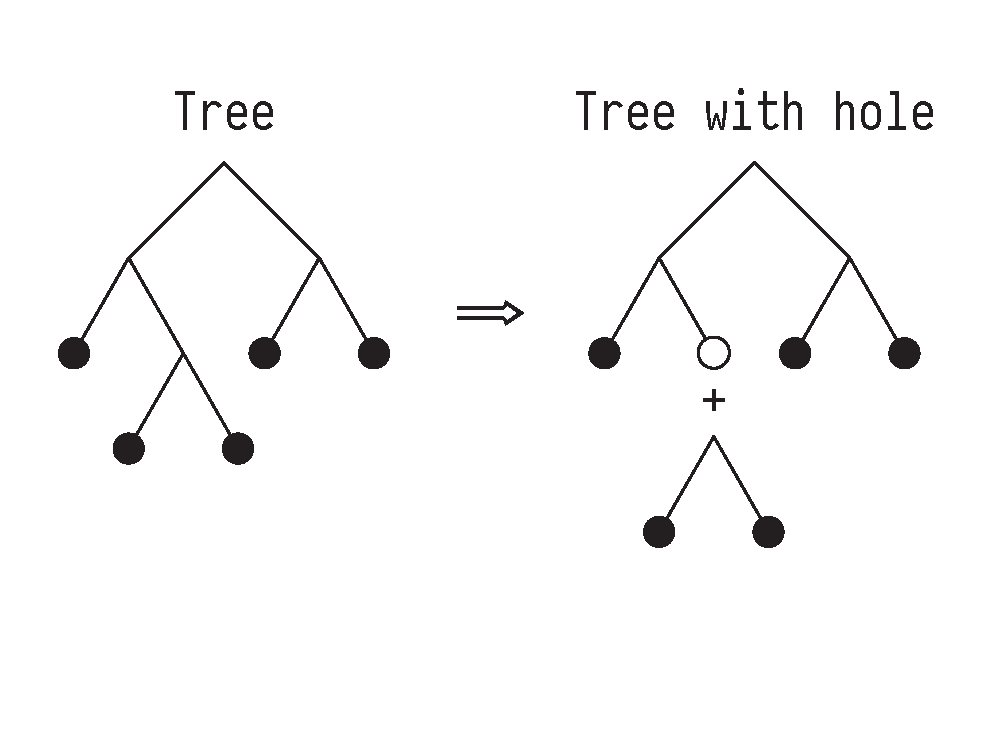
\includegraphics{fig/tree_diff.pdf}
\caption{}
\end{figure}

\end{frame}

\begin{frame}[fragile]{Let's do a simple example}

What is the context for a product type?

\begin{haskellcode}
(x, x) -- sometimes called $x^2$
\end{haskellcode}

\pause

Well we either be focusing on the left side\footnote<.->{here \texttt{○}
  will represent the focus}

\begin{haskellcode}
(○, x)
\end{haskellcode}

\pause

or the right side.

\begin{haskellcode}
(x, ○)
\end{haskellcode}

\pause

We can represent this as \texttt{Either\ (One,\ x)\ (x,\ One)}
(sometimes written as \(2x\)).

\end{frame}

\begin{frame}[fragile]{And now a triple}

What is the context for a triple?

\begin{haskellcode}
(x, x, x) -- sometimes called $x^3$
\end{haskellcode}

\pause

Well we either be focusing on the left side\footnote<.->{here \texttt{○}
  will represent the focus}

\begin{haskellcode}
(○, x, x)
\end{haskellcode}

or the middle

\begin{haskellcode}
(x, ○, x)
\end{haskellcode}

or the right side

\begin{haskellcode}
(x, x, ○)
\end{haskellcode}

\pause

We can represent this as
\texttt{Either\ (Either\ (One,\ x,\ x)\ (x,\ One,\ x))\ (x,\ x,\ One)}
(sometimes written as \(3x^2\)).

\end{frame}

\begin{frame}[fragile]{And the context for One?}

Can we have a one hole context for the \texttt{One} type?

\begin{haskellcode}
data One = One
\end{haskellcode}

\pause

Well we have nothing to take the context of (an \texttt{x}), so we can
represent the context as impossible.

\begin{haskellcode}
data Void
\end{haskellcode}

\end{frame}

\begin{frame}[fragile]{Enumeration Context}

Actually, this trick can be done for any simple enumeration.

\begin{haskellcode}
-- Some enumeration
data Cards = Hearts | Spades | Clubs |Diamonds -- 4
\end{haskellcode}

\pause

\begin{haskellcode}
-- And the context with respect to some variable
data Void
\end{haskellcode}

\end{frame}

\begin{frame}[fragile]{Context for addition}

Say we have the data type

\begin{haskellcode}
data Crafty x = Left x | Right (x, x)
\end{haskellcode}

What is the one hold context for this?

\pause

Well we could either have a hole in the left side, or a hole in one of
two positions on the right side.

\begin{haskellcode}
Either One (Either (One, x) (x, One))
\end{haskellcode}

\end{frame}

\begin{frame}[fragile]{A table of what we have so far}

\begin{longtable}[c]{@{}llll@{}}
\toprule
Type & Number & Context & Number\tabularnewline
\midrule
\endhead
One & 1 & Void & 0\tabularnewline
Cards & 4 & Void & 0\tabularnewline
(x, x) & \(x^2\) & \texttt{(x,\ One)\ :+:\ (One,\ x)} &
\(2x\)\tabularnewline
(x, x, x) & \(x^3\) & \texttt{(One,\ x,\ x)\ :+:\ (x,\ One,\ x)} &
\(3x^2\)\tabularnewline
& & \texttt{:+:\ (x,\ x,\ One)} &\tabularnewline
Crafty & \(x^2 + x\) & \texttt{(x,\ One)\ :+:\ (One,\ x)\ :+:\ One} &
\(2x +1\)\tabularnewline
\bottomrule
\end{longtable}

\pause

That looks an awful lot like differentiation.

\end{frame}

\begin{frame}[fragile]{What else is a differentiation}

What is the differentation of \texttt{{[}a{]}}?

\pause

({[}a{]}, {[}a{]})

\end{frame}

\begin{frame}[fragile]{What have we learned thus far?}

We have learned

\begin{itemize}
\itemsep1pt\parskip0pt\parsep0pt
\item
  how to do algebra on types.
\item
  What a zipper is
\item
  That taking the derivative of a type gives us back a zipper.
\end{itemize}

There are other differentiation laws such as the chain rule for
composition and differentiating a fixed point type.

\end{frame}

\section{Dissection}\label{dissection}

\begin{frame}[fragile]{An example use of a zipper}

Let's look at a binary tree.\footnote<.->{this example stolen wholesale
  from the}

\begin{haskellcode}
data Expr = Val Int | Add Expr Expr

eval :: Expr -> Int
eval (Val x) = x
eval (Add e1 e2) eval e1 + eval e2
\end{haskellcode}

\end{frame}

\begin{frame}[fragile]{Trying a tail recursive version}

\begin{haskellcode}
type Stack = [Expr :+: Int]

eval :: Expr -> Int
eval e = load e []

load :: Expr -> Stack -> Int
load (Val i) stk = unload i stk
load (Add e1 e2_ = load e1 (Left e2 : stk)

unload :: Int -> Stack -> Int
unload v [] = v
unload v1 (Left e2: stk) = load e2 (Right v1 : stk)
unload v2 (Right v1 : stk) = unload (v1 + v2) stk
\end{haskellcode}

\end{frame}

\begin{frame}[fragile]{Eval can be implemented generically two ways}

\begin{itemize}
\itemsep1pt\parskip0pt\parsep0pt
\item
  Differentiating a data type (the Conor McBride method)
\item
  Delimited continuations to pause a traversal (the Oleg Kiselyov
  method)
\end{itemize}

\end{frame}

\begin{frame}[fragile]{Examples}

\begin{itemize}
\itemsep1pt\parskip0pt\parsep0pt
\item
  Folding a tree, finding its maximum path weight, height, etc
\item
  Generating a tree (ex: a Stern-Brocot tree)
\item
  Inverting a tree to perform some action at the leaves (ex: hasSuffix)
\end{itemize}

\end{frame}

\begin{frame}[fragile]{Quote}

``But if there is a message for programmers and programming language
designers, it is this: the miserablist position that types only exist to
police errors is thankfully no longer sustainable, once we start writing
programs like this {[}generic zippers{]}. By permitting calculations of
types and from types, we discover what programs we can have, just for
the price of structuring our data. What joy!''

-- Conor McBride

\end{frame}

\begin{frame}[fragile]{References}

\begin{itemize}
\itemsep1pt\parskip0pt\parsep0pt
\item
  \href{http://strictlypositive.org/CJ.pdf}{Clowns to the Left of me,
  Jokers to the Right} by Conor McBride (the POPL version).
\item
  \href{http://www.slideshare.net/lawrencepaulson/type-classes-slides}{Organizing
  Numerical Theories using Axiomatic Type Classes} by Pawrence Paulson
\item
  \href{https://www.youtube.com/watch?v=YScIPA8RbVE}{The Algebra of
  Albebraic Data Types} by Chris Taylor (written version
  \href{http://chris-taylor.github.io/blog/2013/02/10/the-algebra-of-algebraic-data-types/}{1},
  \href{http://chris-taylor.github.io/blog/2013/02/11/the-algebra-of-algebraic-data-types-part-ii/}{2},
  and
  \href{http://chris-taylor.github.io/blog/2013/02/13/the-algebra-of-algebraic-data-types-part-iii/}{3})
\item
  \href{http://bartoszmilewski.com/2014/10/28/category-theory-for-programmers-the-preface/}{Category
  Theory for Programmers} by Bartosz Milewski
\item
  \href{https://www.fpcomplete.com/user/edwardk/conquering-folds}{Conquering
  Folds} by Edward Kmett
\item
  Zippers Part
  \href{https://pavpanchekha.com/blog/zippers/huet.html}{1},
  \href{https://pavpanchekha.com/blog/zippers/derivative.html}{2},
  \href{https://pavpanchekha.com/blog/zippers/kiselyov.html}{3} by Pavel
  Panchekha
\end{itemize}

\end{frame}

\begin{frame}[fragile]{Extra Stuff}

\begin{haskellcode}
data Tree = Leaf | Node Tree Tree deriving Show

foldTree :: a -> (a -> a -> a) -> Tree -> a
foldTree l n Leaf = l
foldTree l n (Node a b) = n (foldTree l n a) (foldTree l n b)

t = Node (Node Leaf (Node (Node Leaf Leaf) Leaf)) (Node Leaf Leaf)
\end{haskellcode}

\pause

\begin{haskellcode}
foldTail :: forall a. a -> (a -> a -> a) -> Tree -> a
foldTail l n t = inward t []
    where

        inward :: Tree -> [Either Tree a] -> a
        inward Leaf       gamma = outward l gamma
        inward (Node a b) gamma = inward a (Left b:gamma)

        outward :: a -> [Either Tree a] -> a
        outward t [] = t
        outward t (Left b:gamma) = inward b (Right t:gamma)
        outward t (Right u:gamma) = outward (n u t) gamma
\end{haskellcode}

\end{frame}

\end{document}
